\documentclass[tikz,border=4pt]{standalone}
% Shared style for every figure and for the deck: one accent, one
% highlight, thin lines, rounded nodes, nothing decorative.
\usepackage[T1]{fontenc}
\usepackage{lmodern}
\renewcommand{\familydefault}{\sfdefault}
\usepackage{tikz}
\usetikzlibrary{arrows.meta,positioning,calc,shapes.misc,fit,backgrounds,decorations.pathreplacing}
\definecolor{ink}{RGB}{40,40,40}
\definecolor{soft}{RGB}{150,150,150}
\definecolor{faint}{RGB}{225,225,225}
\definecolor{accent}{RGB}{0,95,115}
\definecolor{accentlight}{RGB}{214,232,236}
\definecolor{warn}{RGB}{196,84,40}
\definecolor{warnlight}{RGB}{247,226,216}
\tikzset{
  every picture/.style={color=ink, line width=0.5pt, font=\small},
  node distance=12mm and 18mm,
  box/.style={draw=ink, rounded corners=2pt, fill=white, inner sep=5pt, minimum height=7mm, align=center},
  maker/.style={box, minimum width=18mm},
  cat/.style={box, inner sep=3.5pt, minimum height=6mm},
  root/.style={box, fill=accentlight, draw=accent},
  bad/.style={box, fill=warnlight, draw=warn},
  ghost/.style={box, draw=soft, text=soft, dashed},
  flow/.style={-{Stealth[length=4pt,width=3.5pt]}, line width=0.5pt},
  sub/.style={-{Stealth[length=4pt,width=3.5pt]}, line width=0.5pt, color=soft},
  strong/.style={flow, color=accent, line width=0.8pt},
  wrong/.style={flow, color=warn},
  lbl/.style={font=\footnotesize, text=ink, inner sep=1.5pt, fill=white},
  note/.style={font=\footnotesize, text=soft, align=center},
  rate/.style={font=\footnotesize, text=accent, inner sep=1pt, fill=white},
}

\usepackage{amsmath}
\usepackage{pgfplots}
\pgfplotsset{compat=1.17}

\begin{document}
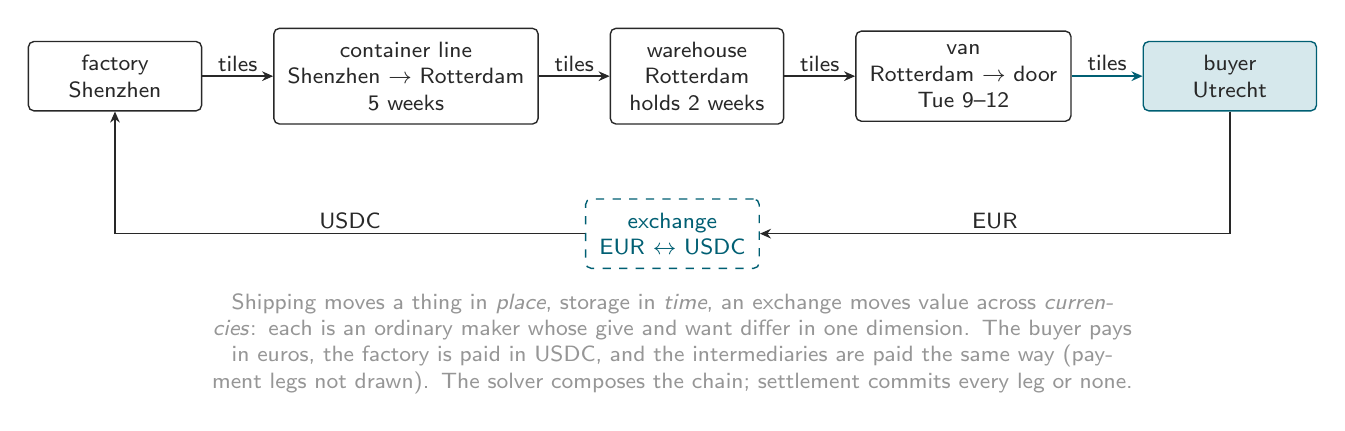
\begin{tikzpicture}[hop/.style={box, align=center, font=\footnotesize, minimum width=22mm}]
  % Longer loops: every intermediary is an ordinary maker whose give and
  % want differ in one dimension -- place (shipping), time (storage),
  % currency (exchange). The solver composes; settlement commits together.
  \node[hop] (F) at (0,0) {factory\\ Shenzhen};
  \node[hop, right=9mm of F] (ship) {container line\\ Shenzhen $\to$ Rotterdam\\ 5 weeks};
  \node[hop, right=9mm of ship] (wh) {warehouse\\ Rotterdam\\ holds 2 weeks};
  \node[hop, right=9mm of wh] (van) {van\\ Rotterdam $\to$ door\\ Tue 9--12};
  \node[hop, right=9mm of van, fill=accentlight, draw=accent] (B) {buyer\\ Utrecht};
  \draw[flow] (F) -- node[lbl, above] {tiles} (ship);
  \draw[flow] (ship) -- node[lbl, above] {tiles} (wh);
  \draw[flow] (wh) -- node[lbl, above] {tiles} (van);
  \draw[strong] (van) -- node[lbl, above] {tiles} (B);
  \node[hop, dashed, draw=accent, text=accent] (X) at ($(F)!0.5!(B) + (0,-20mm)$) {exchange\\ EUR $\leftrightarrow$ USDC};
  \draw[flow] (B) |- node[lbl, pos=0.75, above] {EUR} (X);
  \draw[flow] (X) -| node[lbl, pos=0.25, above] {USDC} (F);
  \node[note, text width=128mm] at ($(X) + (0,-14mm)$) {Shipping moves a thing in \emph{place}, storage in \emph{time}, an exchange moves value across \emph{currencies}: each is an ordinary maker whose give and want differ in one dimension. The buyer pays in euros, the factory is paid in USDC, and the intermediaries are paid the same way (payment legs not drawn). The solver composes the chain; settlement commits every leg or none.};
\end{tikzpicture}
\end{document}
